%TODO: maybe rename this whole into verified boot?!
\section{Komponenten der Systemsicherheit unter
iOS}\label{sec:components-syssec} Eine Kette von aneinander gereihten und
von einander abhängigen Prozessen trägt maßgeblich zur Systemsicherheit bei. Dies berücksichtigt vor allem den
	Startvorgang, die Software Updates - auch von Drittanbietern - und den Secure
	Enclave (siehe \ref{sec:secure_enclave}). Dies stellt sicher, dass alle
	Kernkomponenten, ob Hard- oder Software, möglichst gefeit vor Angriffen sind, ohne dabei die
	Nutzerfreundlichkeit zu beeinflussen. Wenn dabei einer dieser Schritte
	fehlschlägt, unterbricht der Startvorgang und das Gerät wird in den
	Recovery Modus versetzt. Wenn der Boot-ROM nicht geladen werden kann, wird der DFU (Device
	Firmware Upgrade) Modus betreten.\\ 
	Nachfolgend werden die Komponenten welche maßgeblich zur Systemsicherheit und
	an der Wahrung der Integrität dieser beteiligt sind	detailliert vorgestellt und beschrieben.
	
	\begin{figure}[h]
		\centering
		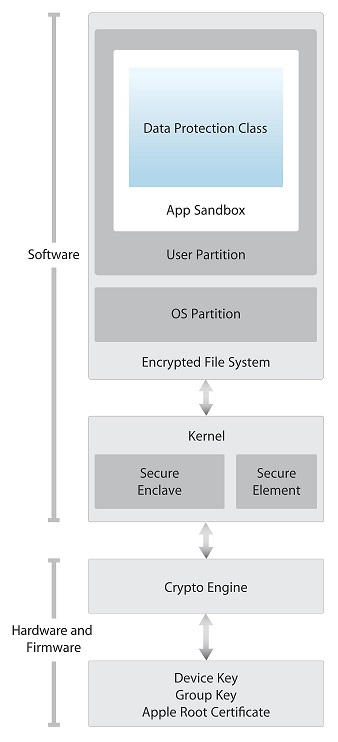
\includegraphics[width=0.4\linewidth]{ios/media/security-model.jpg}
		\caption{Sicherheitsmodel von iOS \cite{iOSSecurityApr2015}}
		\label{fig:security-model}
	\end{figure}

	%TODO: look at learning ios security, there this whole process is explained
	% good
	\subsection{Secure boot chain}\label{sec:secure-boot-chain}
		Dieses Verfahren stellt eine Manipulation der Low-Level Software sicher. Nur
		iOS Geräte, die eine erfolgreiche Validierung dieser Vertrauenskette bestanden
		haben, starten ordnungsgemäß. Dabei wird nach dem Start eines iOS Gerätes
		zuerst Code aus einem nur lesbaren Speicherbereich ausgeführt. Dieser
		\textit{hardware of trust} genannte und unveränderbare Code ist bei der 
		Manufaktur der Chips eingebettet worden und somit implizit vertraulich. Das
		Boot ROM enthält zusätzlich den öffentlichen Schlüssel der Wurzel
		Zertifizierungsstelle von Apple, welcher eine Signierung des
		Low-Level-Bootloaders durch Apple sicher stellt, bevor er ausgeführt wird. 
		Dies ist der erste Schritt in der "`chain of trust"', in welcher jeder
		Teilnehmer sicher stellt, dass der darauf folgende von Apple signiert ist. 		
		Nach erfolgreicher Abarbeitung aller Aufgaben des LLB, überprüft und startet
		dieser iBoot, den nächsten Bootloader, welcher wiederrum das selbe Prozedere
		mit dem iOS Kernel startet. Bei Geräten mit Mobilfunk Zugang führt das
		Basisband Untersystem seinen eigenen ähnlichen Prozess mit signierter 
		Software und verifizierten Schlüsseln vom Basisband Prozessor durch.
		
	\subsection{Authorisierung von System Software}\label{sec:code-signing}
		Dieser Prozess soll einen Downgrade auf eine ältere Version von iOS
		verhindern. Der im folgenden Kapitel besprochene Secure Enclave Co-Prozessor
		nutzt diese Technik für Integritätsprüfung seiner Software ebenfalls. Im Falle
		eines iOS Updates wird entweder von iTunes oder vom Gerät selbst einer der
		Apple Installations Authorisations Server kontaktiert. Diesem wird eine Liste
		von verschlüsselten Messungen pro Komponente, welche am Update
		beteiligt ist, gesandt. Zusätzlich wird ein	zufälliger Anti-Replay Wert und
		die eindeutige ID (ECID) des Gerätes verschickt. Diese Auflistung von gegen
		Versionen, für die ein Update genehmigt ist geprüft. Bei Übereinstimmung wird
		die ECID zu den Messungen hinzugefügt und das Ergebnis signiert, was einer
		Personalisierung der Daten gleicht.	Anschließend werden alle signierten Daten
		zum Gerät geschickt. Die sichere Startkette von Prozessen verifiziert die
		Signatur der empfangenen Daten auf den Absender Apple und ob die Prüfsumme der
		Signatur dem entspricht, was das lokale Ergebnis von verschlüsselten Messungen
		und ECID ergibt.\\
		Mit diesen Schritten wird eine Authorisierung nur für bestimmte Geräte sicher
		gestellt. Außerdem verhindert der Anti-Replay Wert ein mitschneiden der Server
		Antwort und das Verwenden der Daten bei anderen Geräten oder ein manipulieren
		der Daten.
	\subsection{Secure Enclave}\label{sec:secure_enclave}
		%TODO: get more details for ensuring the facts in this chapter
		Dieser Co-Prozessor kommt in Geräten mit A7 oder jüngeren A-Serien Prozessoren
		vor. Er verwendet seinen eigenen sicheren Startvorgang, ist separiert vom
		Applikations Prozessor und verwendet verschlüsselten Speicher, sowie einen
		Hardware Zufallszahlen Generator. Die Technologie basiert auf ARM's
		TrustZone\footnote{http://www.arm.com/products/processors/technologies/trustzone/index.php}
		und wurde von Apple für die eigenen Ansprüche angepasst. Der Kernel dieser
		Einheit basiert auf der L4
		Mikrokernel-Familie\footnote{http://os.inf.tu-dresden.de/L4/} mit leichten
		Modifikationen. Die auf Interrupts basierende Kommunikation zwischen dem Applikationsprozessor und dem Secure Enclave (SE) läuft über
		einem nur den beiden zur Verfügung stehenden Speicherbereich. Der SE ist
		verantwortlich für das Schlüssel Management der Datenverschlüsselung und
		stellt die Integrität dieser sicher, auch wenn der Kernel des iOS Systems
		kompromitiert ist. Beim Herstellungsprozess erhält jeder SE eine einzigartige
		ID (UID), auf welche nur er zugreifen kann und welche auch Apple selbst nicht
		bekannt ist. Mit dieser UID wird beim Systemstart der Speicherbereich des SE
		zusammen mit einem einmaligen Schlüssel verschlüsselt. Zusätzlich werden
		jegliche vom SE in den Speicher geschriebene Daten mit der UID und einem
		Anti-Replay Zufallswert verschlüsselt. Eine der Hauptaufgaben des Secure
		Enclave ist die verarbeitung der Fingerabdruck-Daten des Touch
		ID (siehe: \ref{sec:touch_id}). Alle Kommunikation zwischen Touch ID und SE
		wird über einen seriellen Bus abgearbeitet. Der Applikationsprozessor leitet die Fingerabdrucksdaten an den
		SE weiter kann diese aber aufgrund einer Verschlüsselung der Daten mit einem
		Sitzungsschlüssel nicht lesen. Dieser Session Key wurde durch den für Touch ID
		und SE bereit gestellten öffentlichen Schlüssel erzeugt. Der Austausch des
		Sitzungsschlüssels wird durch AES Key Wrapping realisiert. Dabei erzeugen
		beide Seiten einen zufälligen Schlüssel, welche den Sitzungsschlüssel bilden.
		Zum verschlüsselten Transport wird AES-CCM genutzt.
	\subsection{Touch ID}\label{sec:touch_id}
		Touch ID bezeichnet den Fingerabdrucksensor der in allen iPhone 5s und neuer
		, sowie iPad Air 2 und iPad mini 3 verbaut ist. Es können bis zu 5
		Fingerabdrücke gespeichert werden. Eine der größten Vorteile dabei ist das
		sofortige Sperren des Gerätes beim drücken des Sleep/Wake-Buttons. Vor der
		Einführung von Touch ID haben viele Nutzer eine möglichst lange Zeit
		eingestellt, bis das Eingeben des Passcodes nötig wurde, nachdem das Gerät
		gesperrt wurde. Dies entfällt bei aktiviertem Touch ID nun, da man nur noch
		mit seinem Finger Entsperren muss. Touch ID kann zusätzlich zum
		Entsperren des Gerätes auch mit dem Zahlungsdienst Apple Pay und für Einkäufe
		in iTunes, dem App Store und im iBook Store genutzt werden. Für Entwickler
		steht eine API bereit mit der aber rudimentärste Prüfungen auf erfolgreiche
		Verifikation des Abdrucks erfolgen können. Ein direkter Zugriff auf Touch ID
		oder die Daten des Fingerabdrucks wird von Apple unterbunden. Touch ID wird
		aktiviert, wenn der kapazitive Stahlring um den Sensor einen Fingerdruck
		wahrnimmt. Dann wird dieser gescannt und an den Secure Enclave geschickt. Der
		Abdruck wird kurzzeitig im veschlüsselten Speicher des SE gespeichert um die
		Daten zu Vektorisieren, danach wird dieser verworfen. Die Schlüssel, welche
		von Touch ID zum Entschlüsseln des Gerätes benötigt werden, sind nach 48
		Stunden ungültig, bzw. wenn das iOS Gerät neu gestartet wurde, oder der
		Fingerabdruck fünf mal falsch registriert wurde.\\
		Dass diese Technik nicht als Sicher angesehen werden darf, haben bereits
		Miglieder des Chaos Computer Club gezeigt
		\footnote{http://www.ccc.de/de/updates/2013/ccc-breaks-apple-touchid}, dabei 
		wurde mit simpelsten Haushaltsmitteln ein Fingerabdruck gefälscht, den das
		Smartphone irrtümlicher weise akzeptiert hat.
